\begin{figure}[H]
    \centering
    \setlength{\unitlength}{\textwidth}
    \vspace{-5mm}
    \begin{picture}(1,.75)
        \put(0,0){\includegraphics[width=\unitlength]{plot1.eps}}%
        \put(0.4,0.55){$f(x) = \sqrt{x}$}
        \put(0.35,0.37){$g(x) = \sin{x}$}
        \put(0.14,0.40){$h(x) = e^{-x^2}$}
    \end{picture}%
    \vspace{-10mm}
    \caption{Overlaying \LaTeX\ commands on top of the figure.}
    \label{fig:plot2}
\end{figure}
